\chapter{Охрана труда и экология}
\section{Проектирование рабочего места оператора ПЭВМ}
Требования к компьютерной технике и к условиям работы с ней в Российской Федерации регламентируются санитарными нормами и правилами СанПиН 2.2.2/2.4.1340-03 и СанПиН 2.2.2.000-02. Рассмотрим основные нормы, необходимые для проектирования рабочего места оператора ПЭВМ.

\subsection{Требования к рабочим помещениям}
Согласно СанПиН 2.2.2/2.4.1340-03, помещения для работы с компьютерами должны оборудоваться системами отопления, кондиционирования воздуха или эффективной приточно-вытяжной вентиляцией. Звукоизоляция помещений и звукопоглощение ограждающих конструкций помещения должны отвечать гигиеническим требованиям и обеспечивать нормируемые параметры шума на рабочих местах. Помещения должны иметь естественное и искусственное освещение.

Поверхность пола в помещениях должна быть ровной, без выбоин, нескользкой, удобной для очистки и влажной уборки, обладать антистатическими свойствами. При строительстве новых и реконструкции действующих средних, средних специальных и высших учебных заведений помещения для работы с компьютером следует проектировать высотой (от пола до потолка) не менее 4,0 м.

Расположение рабочих мест для взрослых пользователей в подвальных помещениях не допускается.

\subsection{Требования к освещению}
Естественное освещение должно осуществляться через светопроемы, ориентированные преимущественно на север и северо-восток. Оконные проемы в помещениях использования компьютеров должны быть оборудованы регулируемыми устройствами типа жалюзи, занавесей, внешних козырьков и др. Система естественного освещения должна обеспечивать коэффициент естественной освещенности (КЕО) не ниже 1,5.

Искусственное освещение в помещениях должно осуществляться системой общего равномерного освещения. В производственных и административно - общественных помещениях, в случаях преимущественной работы с документами, допускается применение системы комбинированного освещения (к общему освещению дополнительно устанавливаются светильники местного освещения, предназначенные для освещения зоны расположения документов). 

Освещенность на поверхности стола в зоне размещения рабочего документа должна быть 300-500~лк. Допускается установка светильников местного освещения для подсветки документов. Местное освещение не должно создавать бликов на поверхности экрана и увеличивать освещенность экрана более 300~лк. 

Следует ограничивать прямую блескость от источников освещения, при этом яркость светящихся поверхностей (окна, светильники и др.), находящихся в поле зрения, должна быть не более 200~кд/кв. м. В качестве источников света при искусственном освещении должны применяться преимущественно люминесцентные лампы типа ЛБ. При устройстве отраженного освещения в производственных и административно-общественных помещениях допускается применение металлогалогенных ламп мощностью до 250 Вт. Допускается применение ламп накаливания в светильниках местного освещения. 

Для освещения помещений следует применять светильники серии ЛПО36 с зеркализованными решетками, укомплектованные высокочастотными пускорегулирующими аппаратами (ВЧ ПРА). Коэффициент пульсации не должен превышать 5\%, что должно обеспечиваться применением газоразрядных ламп в светильниках общего и местного освещения с ВЧ ПРА. 

Допускается применять светильники серии ЛПО36 без ВЧ ПРА только в модификации «Кососвет», а также светильники прямого света -- П, преимущественно прямого света -- Н, преимущественно отраженного света -- В. При этом лампы многоламповых светильников или рядом расположенные светильники общего освещения следует включать на разные фазы трехфазной сети.

Применение светильников без рассеивателей и экранирующих решеток не допускается. Яркость светильников общего освещения в зоне углов излучения от 50\textdegree до 90\textdegree с вертикалью в продольной и поперечной плоскостях должна составлять не более 200 кд/кв. м, защитный угол светильников должен быть не менее 40\textdegree. Светильники местного освещения должны иметь непросвечивающий отражатель с защитным углом не менее 40\textdegree.

Для обеспечения нормируемых значений освещенности в помещениях использования ВДТ и ПЭВМ следует проводить чистку стекол оконных рам и светильников не реже двух раз в год и проводить своевременную замену перегоревших ламп.

Коэффициент запаса (Кз) для осветительных установок общего освещения должен приниматься равным 1,4. 

Для внутренней отделки интерьера помещений должны использоваться диффузно-отражающие материалы с коэффициентом отражения 
\begin{itemize}
	\item для потолка $\rho_{\pe\co\te} = 0,7-0,8$;
	\item для стен $\rho_{\es\te} = 0,5-0,6$;
	\item для пола $\rho_{\pe\co\el} = 0,3-0,5$;
\end{itemize}

\subsection{Расчёт системы освещения в помещении}

В помещении, где находится рабочее место оператора, используется смешанное освещение, т.е. сочетание естественного и искусственного освещения. В качестве естественного -- боковое освещение через окно. Искусственное освещение используется при недостаточном естественном освещении. В данном помещении используется общее искусственное освещение.

Расчет его осуществляется по методу светового потока с учетом потока, отраженного от стен и потолка.

Нормами для данных работ установлена необходимая освещенность рабочего места $E_{\en}=300\el\ka$ (средняя точность работы по различению деталей размером от 1 до 10 мм). 

Площадь помещения:
\begin{equation*}
	S = A \cdot B = 4 \cdot 6 = 24 \cm.
\end{equation*}

Общий световой поток определяется по формуле:
\begin{equation*}
	F = \frac{E \cdot K \cdot S \cdot Z}{n},
\end{equation*}
где $E$ -- нормированная минимальная освещённость, лк. Работа программиста относится к разряду точных работ, следовательно, минимально освещённость будет $E = 300 \el\ka$ при газоразрядных лампах;

$Z$ -- отношение средней освещённости к минимальной (обычно принимается равным $1,1-1,2$, положим $Z = 1,1$);

$K$ -- коэффициент запаса, учитывающий уменьшение светового потока лампы в результате загрязнения светильников в процессе эксплуатации (его значение определяется по таблице коэффициентов запаса для различных помещений и в нашем случае $К = 1,5$);

$n$ -- коэффициент использования (выражается отношением светового потока, падающего на расчетную поверхность, к суммарному потоку всех ламп и исчисляется в долях единицы; зависит от характеристик светильника, размеров помещения, окраски стен и потолка, характеризуемых коэффициентами отражения от стен $P_c$ и потолка $P_{\pe}$). Значение коэффициентов $P_c$ и $P_{\pe}$ определим по таблице зависимостей коэффициентов отражения от характера поверхности: $P_c=30\%$, $P_{\pe}=50\%$. Значение $n$ определим по таблице коэффициентов использования различных светильников. Для этого вычислим индекс помещения по формуле:
\begin{equation*}
	I = \frac{S}{h \cdot (A + B)},
\end{equation*}
где $S$ -- площадь помещения, $S = 24 \cm^2$;

$h$ -- расчётная высота подвеса, $h = 3 \cm$;

$A$ -- длина помещения, $A = 6 \cm$;

$B$ -- ширина помещения, $B = 4 \cm$.

Подставив значения, получим:

\begin{equation*}
	I = \frac{24}{3 \cdot (6 + 4)} = 0,8
\end{equation*}

Зная индекс $i$, $P_c$, $P_{\pe}$, по таблице находим, что значения $n = 0,36$.

Подставим все значения в формулу для определения светового потока $F$:

\begin{equation*}
	F = \frac{300 \cdot 1,5 \cdot 24 \cdot 1,1}{0,36} = 33000 \el\cm
\end{equation*}

Люминесцентные лампы имеют ряд преимуществ перед лампами накаливания: их спектр ближе к естественному, обладают более высоким КПД (в 1,5-2 раза выше, чем КПД ламп накаливания), имеют большую экономичность (больше светоотдача) и срок службы (в 10-12 раз). Наряду с этим имеются и недостатки: их работа сопровождается иногда шумом; хуже работают при низких температурах; их нельзя применять во взрывоопасных помещениях; имеют малую инерционность. Для нашего помещения люминесцентные лампы подходят.

Для освещения выбираем люминесцентные лампы типа ЛБ40-1, световой поток которых F = 4320 лм. 

Рассчитаем необходимое количество ламп по формуле:

\begin{equation*}
	N = \frac{F}{F_{\EL}},
\end{equation*}
где $N$ -- определяемое число ламп;

$F$ -- световой поток, $F = 33000 \el\cm$;

$F_{\el}$ -- световой поток лампы, $F_{\el} = 4320 \el\cm$.

\begin{equation*}
	N = \frac{33000}{4320} = 8 \csh\te.
\end{equation*}

При выборе осветительных приборов используем светильники типа ОД. Каждый светильник комплектуется двумя лампами ЛБ40. Размещаются светильники двумя рядами, по два в каждом ряду.

Рассчитаем суммарную мощность осветительной установки общего назначения:

\begin{equation*}
	P \sum = 40 \cdot 16 = 640 \VE\te.
\end{equation*}

\subsection{Требования к микроклимату}

Оптимальным температурным режимом работы принимается температура окружающей среды от 19\textdegree до 21\textdegree и соответствующие им значения относительной влажности от 62\% до 55\%. Абсолютная влажность воздуха должна быть около 10г/$\cm^3$. Скорость движения воздуха требуется ограничить значением менее 0,1 м/с . Для наиболее производительной и успешной работы инженера-программиста (пользователя ПЭВМ), требуется обеспечить характеристики микроклимата по значениям, не уступающим вышеизложенным.

Вышеуказанные требования СанПиН были соблюдены на рабочем месте, где проходило выполнение данного дипломного проекта. Система отопления включала основную и вспомогательную системы. Основная система – система приточной вентиляции с подогревом воздуха, также выполняющая роль системы вентиляции помещения. Вспомогательная – статический обогрев помещения за счет батарей центрального отопления. Контроль за соблюдением техники безопасности и удовлетворением норм микроклимата регулярно проводится инженером по технике безопасности. Рабочее место аттестовано сертифицированными службами и допущено к эксплуатации.

\section{Расчёт системы вентиляции}
Помещения, в которых производится эксплуатации ПЭВМ, должны быть оборудованы системами приточно-вытяжной вентиляции, при работе которой будут обеспечены допустимые параметры микроклимата в помещении. Расчет производят только для вытяжной ветви приточно-вытяжной системы вентиляции.

$V_{\ve\e\en\te}$ -- объем воздуха, необходимый для обмена, $\cm^3$/ч;
$V_{\pe\co\cm}$ -- объем рабочего помещения, $\cm^3$.
Для расчета примем следующие размеры рабочего помещения: 
\begin{itemize}
	\item длина $В = 6 \cm$; 
	\item ширина $А = 4 \cm$; 
	\item высота $Н = 3 \cm$. 
\end{itemize}

Соответственно, объем помещения равен: 
\begin{equation*}
	V_{\pe\co\cm} = A \cdot B \cdot H = 72 \cm^3.
\end{equation*}

Необходимый для обмена объём воздуха $V_{\ve\e\en\te}$ определим исходя из уравнения теплового баланса:
\begin{equation*}
	V_{\ve\e\en\te} \cdot (t_{\cu\ha\co\de} - t_{\pe\re\ci\ha\co\de}) \cdot Y = 3600 \cdot Q_{\ci\ze\be},
\end{equation*}
где $Q_{\ci\ze\be}$ -- избыточная теплота (Вт);

$C = 1005 \DE\zhe / (\ka\ge \cdot \KA)$ -- удельная теплопроводная воздуха;

$Y = 1,2 \cm\ge / \es\cm^3$ -- плотность воздуха.

Температура уходящего воздуха определяется по формуле:
\begin{equation*}
	t_{\cu\ha\co\de} = t_{\re\cm} + (H - 2) \cdot t,
\end{equation*}
где $t = 1-5^\circ$ -- превышение t на 1м высоты помещения;

$t_{\re\cm} = 21^\circ$ -- температура на рабочем месте;

H = $3 \cm$ -- высота помещения;

\begin{eqnarray*}
	t_{\cu\ha\co\de} = 21 + (3 - 2) \cdot 4,7 = 25,47^\circ \\
	Q_{\ci\ze\be} = Q_{\ci\ze\be1} + Q_{\ci\ze\be2} + Q_{\ci\ze\be3},
\end{eqnarray*}
где $Q_{\ci\ze\be}$ -- избыток тепла от электрооборудования и освещения.

\begin{equation*}
	Q_{\ci\ze\be1} = E \cdot p
\end{equation*}
где $E$ -- коэффициент потерь электроэнергии на теплоотвод ($E = 0,55$ для освещения);

$p$ -- мощность, $p = 40 \VE\te \cdot 8 + 500 \VE\te = 820\VE\te$.
\begin{equation*}
	Q_{\ci\ze\be1} = 0,55 \cdot 820 = 461 \VE\te,
\end{equation*}
$Q_{\ci\ze\be2}$ -- теплопоступление от солнечной радиации,
\begin{equation*}
	Q_{\ci\ze\be2} = m \cdot S \cdot k \cdot Q_c,
\end{equation*}
где $m$ -- число окон, примем $m = 2$;

$S$ -- площадь окна, $S = 2,2 \cdot 1,5 = 3,3 \cm^2$;

$k$ -- коэффициент, учитывающий остекление (для двойного остекления $k = 0,6$);

$Q_c = 127 \VE\te / \cm$ -- теплопоступление от окон.

\begin{equation*}
	Q_{\ci\ze\be2} = 3,3 \cdot 2 \cdot 0,6 \cdot 127 = 505,92 \VE\te.
\end{equation*}

$Q_{\ci\ze\be3}$ -- тепловыделение людей.

\begin{equation*}
	Q_{\ci\ze\be3} = n \cdot q,
\end{equation*}
где $q = 80 \VE\te / \che\e\el.$,

$n$ -- число людей ($n = 1$).

Тогда

\begin{eqnarray*}
	Q_{\ci\ze\be3} = 1 \cdot 80 = 80 \VE\te \\
	Q_{\ci\ze\be} = 461 + 502 + 80 = 1143 \VE\te
\end{eqnarray*}

Из уравнения теплового баланса следует:

\begin{equation*}
	V_{\ve\e\en\te} = \frac{3600 \cdot 1143}{1005 \cdot 1,2 \cdot (25,47 - 19)} = 527,35 \cm^3 / \che\ca\es
\end{equation*}

\subsection{Выбор вентилятора}
В нашем случае будет использоваться приточно-вытяжная вентиляция.

Вентиляционная система состоит из следующих элементов (рисунок~\ref{img:ventilation}): 
\begin{enumerate}
	\item забор воздуха;
	\item система кондиционирования;
	\item вентилятор;
	\item решетка;
	\item стальной воздуховод с круглым сечением;
	\item стальной воздуховод с круглым сечением;
	\item выброс воздуха.
\end{enumerate}

\begin{figure}[H]
    \center{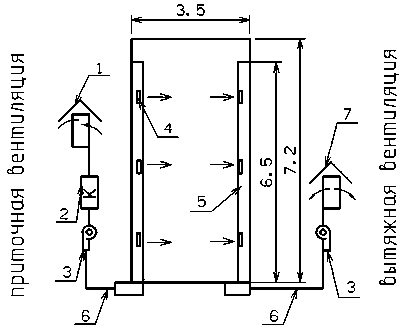
\includegraphics[width=0.5\linewidth]{ventilation}}
    \caption{Вентиляционная система.}
    \label{img:ventilation}
\end{figure}

Исходными данными для выбора вентилятора является расчётная производительность вентилятора:

\begin{equation*}
	V_{\re\ca\es\che} = 1,1 \cdot V_{\ve\e\en\te} = 1,1 \cdot 527 = 579,7 \cm^3 / \che\ca\es,
\end{equation*}
где $1,1$ -- коэффициент, учитывающий утечки и подсосы воздуха.

Потери давления в вентиляционной системе определяются по формуле:
\begin{equation*}
	H = R \cdot l + \xi \cdot \frac{V^2 \cdot p}{2},
\end{equation*}
где $H$ -- потери давления, Па;

$R$ -- увдельные потери давления на трение в воздуховоде, Па/м;

$I = 4,5 \cm$ -- длина воздуховода;

$V = 7 \cm / \es$ -- скорость воздуха;

$p = 1,2 \ka\ge / \cm$ -- плотность воздуха.

Необходимый диаметр воздуховода для данной вентиляционной системы:

\begin{equation*}
	L = \frac{d^2 \cdot \pi}{4} \cdot W,
\end{equation*}
где $L = V_{\re\ca\es\che} = 579,7 \cm^3 / \che\ca\es$;

$W = 7 \cm / \es$.

\begin{equation*}
	d = \sqrt{ \frac{4 \cdot L}{\pi \cdot W}} = 0,17 \cm.
\end{equation*}

Принимаем в качестве диаметра ближайшую большую стандартную величину -- 0,2 м, при которой удельные потери давления на трение в воздуховоде -- $R = 3,58 \PE\ca / \cm$.

После перехода на стандартный диаметр производим перерасчёт скорости:

\begin{equation*}
	W_{\en\co\re} = \frac{4}{d^2 \cdot \pi} \cdot L = 5,12 \cm / \es.
\end{equation*}

Местные потери возникают в железной решётке ($\xi = 1,2$), в изгибе трубопровода ($\xi = 1,7$). Отсюда суммарный коэффициент местных потерь в системе:

\begin{equation*}
	\xi = (1,2 \cdot 3) + 1,7 = 5,3.
\end{equation*}

Тогда

\begin{equation*}
	 H = 3,58 \cdot 4,5 + 5,3 \cdot \frac {26,2 \cdot 1,2}{2} = 99,4 \PE\ca.
\end{equation*}

С учётом 10\% запаса:

\begin{equation*}
	H = 1,1 \cdot 99,4 = 109,3 \PE\ca.
\end{equation*}

Далее в проводимом расчёте по вычисленному напору определяется марка вентилятора из соответствующих таблице. Рассмотрим, например, соответствующую таблицу для вентиляторов радиальных (центробежных) серии ВЦ-4-70 (таблица~\ref{tab:fans}).

\begin{table}[H]
    \caption{\label{tab:fans} Вентиляторы радиальные (центробежные) серии ВЦ-4-70.}
    \begin{center}
        \begin{tabular}{|l|c|c|c|c|c|c|c|c|}
            \hline
             &
            \multicolumn{2}{|c|}{Электродвигатель} &
            \multicolumn{2}{|c|}{\specialcell{Характеристики\\вентилятора}} &
            \multicolumn{4}{|c|}{Исполнение}\\
            \cline{2-9}
            \raisebox{-1ex}[5cm][0cm]{\specialcell{Марка\\вент.}} &
            \specialcell{Мощность,\\кВт} &
            \specialcell{Частота\\вращения,\\об./мин.} &
            \specialcell{Расход\\воздуха,\\$\cm^3 \cdot 10^3$/час} &
            \specialcell{Напор,\\Па} &
            \rotatebox{90}{\specialcell{Обычное}} &
            \rotatebox{90}{\specialcell{Коррозионноестойкое}} &
            \rotatebox{90}{\specialcell{Искрозащищённое}} &
            \rotatebox{90}{\specialcell{Взрывозащищённое}} \\
            \hline
            \multirow{2}{*}{\specialcell{ЦВ-4-\\70-2,5}} &
            0,18 & 1500 & 0,37-0,92 & 140-190 & + & + & + & + \\
             & 0,75 & 3000 & 0,75-1,92 & 500-760 & + & + & + & + \\
            \hline
            \multirow{2}{*}{\specialcell{ЦВ-4-\\70-3,15}} &
            0,27 & 1500 & 0,78-2,0 & 190-310 & + & + & + & + \\
             & 1,5 & 3000 & 1,65-4,10 & 800-1300 & + & + & + & + \\
            \hline
            \multirow{3}{*}{\specialcell{ЦВ-4-\\70-4}} &
            0,18 & 950 & 1,15-2,6 & 130-220 & + & + & + & + \\
             & 1,1 & 1500 & 1,85-4,0 & 300-490 & + & + & + & + \\
             & 7,5 & 3000 & 3,6-7,2 & 1200-2250 & + & + & + & + \\
            \hline
            \multirow{2}{*}{\specialcell{ЦВ-4-\\70-5}} &
            0,55 & 950 & 2,3-5,1 & 160-360 & + & + & + & + \\
             & 2,2 & 1500 & 3,5-8,0 & 380-840 & + & + & + & + \\
            \hline
            \multirow{2}{*}{\specialcell{ЦВ-4-\\70-6,3}} &
            1,5 & 950 & 4,2-10,2 & 310-500 & + & + & + & + \\
             & 5,5 & 1500 & 7,0-16,0 & 580-1280 & + & + & + & + \\
            \hline
        \end{tabular}
    \end{center}
\end{table}

По этим данным выбираем вентилятор ВЦ-4-70-2,5:
\begin{itemize}
	\item расход воздуха: $370-920 \cm^3 / \che\ca\es$;
	\item давление: 140-190 Па;
	\item скорость вращения: 1500 об./мин.;
	\item мощность электродвигателя: 0,18 кВт.
\end{itemize}

\subsection{Требования к размещению оборудования}
Площадь на одно рабочее место с компьютером для взрослых пользователей должна составлять не менее $6,0 \cm^2$, а объем -- не менее $20,0 \cm^2$. Площадь на одно рабочее место с компьютером во всех учебных и дошкольных учреждениях должна быть не менее $6,0 \cm^2$, а объем -- не менее $24,0 \cm^3$.

Рабочие места по отношению к световым проемам должны располагаться так, чтобы естественный свет падал сбоку, преимущественно слева. Схемы размещения рабочих мест с ВДТ и ПЭВМ должны учитывать расстояния между рабочими столами с видеомониторами (в направлении тыла поверхности одного видеомонитора и экрана другого видеомонитора), которое должно быть не менее $2,0 \cm$, а расстояние между боковыми поверхностями видеомониторов -- не менее $1,2 \cm$.

Рабочие места в помещениях с источниками вредных производственных факторов должны размещаться в изолированных кабинах с организованным воздухообменом. Рабочие места с ВДТ и ПЭВМ при выполнении творческой работы, требующей значительного умственного напряжения или высокой концентрации внимания, следует изолировать друг от друга перегородками высотой $1,5 - 2,0 \cm$.

Размещение оборудования на рабочих столах должно отвечать следующим требованиям.

При работе с монитором в глазу происходят процессы аккомодации и конвергенции. Аккомодация -- изменение геометрии хрусталика, при котором изображение фокусируется на сетчатке. Раньше считалось, что расслабление мышц глаза и хрусталика происходит, когда глаз смотрит в бесконечность. Более свежие данные говорят о том, что расслабление соответствует фокусировке на «мнимый» объект на расстоянии примерно 800 мм. Мышцы, поворачивающие глазные яблоки в процессе конвергенции тоже находятся в постоянном напряжении. Новые данные говорят о том, что расслабление глазодвигательных мышц происходит при сведении глазных яблок на «мнимый» объект, удаление которого зависит от угла зрения. Пристальный взгляд под углом 30\textdegree расслабляет глазодвигательные мышцы при удалении предмета на 530 мм. Поэтому экран видеомонитора должен находиться на расстоянии 600-700 мм от глаз пользователя на высоте его головы.

Зона досягаемости составляет 350-400 мм. Ближней зоне соответствует область, охватываемая рукой при прижатом к туловищу локте, дальней зоне -- область вытянутой руки. Поэтому клавиатуру следует располагать на поверхности стола на расстоянии 100-300 мм от края, обращенного к пользователю или на специальной выдвижной панели стола.

На основе данных о физиологии человека были разработаны оптимальные параметры элементов рабочего места, которые в настоящее время стандартизированы и включены в санитарно-гигиенические и эргономические нормативные документы. Для того чтобы обеспечивать свободную и удобную рабочую позу (оптимальные условия труда) элементы рабочего места должны удовлетворять требованиям СанПиН 2.2.2/2.4.1340-03. В табл.~\ref{tab:workplace} приведены оптимальные размеры основных элементов рабочего места (рабочий стол и стул).

\begin{center}
    \begin{longtable}{|l|l|r|r|}
	    \caption{\label{tab:workplace} Параметры оптимального рабочего места пользователя ПК.} \\
            \hline
            \specialcell{Элемент рабочего\\места} &
            \specialcell{Параметры} &
            \specialcell{Величина\\(мм)} &
            \specialcell{Диапазон\\рег-я\\(мм)} \\
            \hline
            \endfirsthead
            
            \hline
            \specialcell{Элемент рабочего\\места} &
            \specialcell{Параметры} &
            \specialcell{Величина\\(мм)} &
            \specialcell{Диапазон\\рег-я\\(мм)} \\
            \hline
            \endhead
            
            \hline
            \endfoot

            \hline
            \endlastfoot

            \multirow{6}{*}{Рабочий стол} &
            \specialcell{Высота рабочей\\поверхности} &
            725 & 680-800 \\
             & Ширина & \specialcell{800, 1000,\\1200, 1400} & нет \\
             & Пространство для ног & & \\
             & \specialcell{высота} & 600 & нет \\
             & \specialcell{глубина на уровне колен} & 450 & нет \\
             & \specialcell{глубина на уровне\\вытянутых ног} & 650 & нет \\
            \hline
			\multirow{12}{*}{\specialcell{Рабочий стул (подъёмно-\\поворотный)}} &
            \specialcell{Ширина сиденья} &
            400 & нет \\
             & Глубина сиденья & \specialcell{400} & нет \\
             & \specialcell{Высота поверхности\\сиденья} & 475 & 400-550 \\
             & \specialcell{Угол наклона сиденья} &  & \\
             & \specialcell{вперёд} & 0\textdegree & 0\textdegree-15\textdegree \\
             & \specialcell{назад} & 0\textdegree & 0\textdegree-15\textdegree \\
             & \specialcell{Высота опорной пов-ти\\спинки} & 300 & 280-320 \\
             & \specialcell{Ширина спинки} & 380 & нет \\
             & \specialcell{Радиус кривизны спинки\\в гор. плоскости} & 400 & нет \\
             & \specialcell{Угол наклона спинки \\в вертикальной\\плоскости} & 0\textdegree & \specialcell{от -30\textdegree\\до +30\textdegree} \\
             & \specialcell{Расстояние от переднего\\края сиденья до спинки} & 330 & 260-400 \\
            \hline
            \multirow{5}{*}{\specialcell{Подлокотники\\(съёмные или\\стационарные)}} & Длина & 250 & нет \\
             & Ширина & 50-70 & нет \\
             & \specialcell{Высота над сиденьем} & 230 & 200-260 \\
             & \specialcell{Расстояние между\\подлокотниками} & 425 & 350-500 \\
            \hline
            \multirow{5}{*}{\specialcell{Подставка\\для ног}} & Ширина & 300 & нет \\
             & Глубина & 400 & нет \\
             & Высота & 150 & нет \\
             & \specialcell{Наклон опорной\\поверхности} & 0\textdegree & 0\textdegree-20\textdegree \\
            \hline
    \end{longtable}
\end{center}

Исходя из данных таблицы, приведём параметры стола программиста:
\begin{itemize}
	\item высота стола -- 725 мм;
	\item длина стола -- 1200 мм;
	\item ширина стола -- 800 мм;
	\item глубина стола -- 400 мм;
	\item поверхность для письма: \begin{itemize}
			\item в глубину -- 40 мм;
			\item в ширину -- 600 мм;
		\end{itemize}
\end{itemize}

\subsection{Требования к мониторам}
Изображение на экране монитора может быть охарактеризовано широким набором параметров. С точки зрения безопасности, первостепенную роль имеют факторы, определяющие характер зрительной работы и вызывающие усталость и нагрузку на зрительный аппарат пользователя компьютера. Эти факторы называются визуальными эргономическими параметрами. К ним относится яркость изображения, четкость изображения,  размер знаков, отклонение положения знаков, искажения изображения, мерцание изображения. К визуальным параметрам также относится отражательная способность экрана, обрамления экрана и корпуса монитора. В таблице~\ref{tab:visual} приведены описания нормируемых параметров и их оптимальные значения.

\begin{center}
    \begin{longtable}{|l|l|l|}
	    \caption{\label{tab:visual} Визуальные эргономические параметры по СанПиН 2.2.2/2.4.1340-03.} \\
            \hline
            Параметр & Описание и определение & \specialcell{Допустимое\\значение} \\
            \hline
            \endfirsthead
            Параметр & Описание и определение & \specialcell{Допустимое\\значение} \\
            \hline
            \endhead

            \endfoot

            \endlastfoot

            \specialcell{Яркость\\изображения} & \specialcell{Яркость знака или фона,\\измерененная в темноте} & от 35 до 120 кд/$\cm^2$ \\ 
            \hline
            \specialcell{Чёткость\\изображения} & \specialcell{Размер минимального\\элемента (зерна)\\изображения} & не более 0,3 мм \\
            \hline
            \multirow{2}{*}{\specialcell{Размер знаков}} & \specialcell{Отношение ширины знака к\\его высоте для прописных\\букв} & \specialcell{от 0,7 до 0,9\\оптимально} \\
             &  & \specialcell{от 0,5 до 1,0\\допустимо} \\
            \hline
            \multirow{2}{*}{\specialcell{Отклонение\\положения\\знаков}} & \specialcell{Допустимое горизонтальное\\смещение однотипных знаков\\в \% от ширины знака} & не более 5 \\
             & \specialcell{Допустимое вертикальное\\смещение однотипных\\знаков в \% от высоты знака} & не более 5 \\
            \hline
            \multirow{3}{*}{\specialcell{Отклонение формы\\рабочего поля\\экрана}} & \specialcell{По горизонтали:\\$\Delta B = \frac{2(B_1 - B_2)}{(B_1 + B_2)} $} & $\Delta B \le 0,02 $ \\
             & \specialcell{По вертикали:\\$\Delta H = \frac{2(H_1 - H_2)}{(H_1 + H_2)}$} & $\Delta H \le 0,02 $ \\
             & \specialcell{По диагонали:\\$\Delta D = \frac{2(D_1 - D_2)}{(D_1 + D_2)}$} & $\Delta D \le 0,04 \cdot (H_1 - H_2) $ \\
            \hline
            \specialcell{Мерцание\\изображения} & \specialcell{Допустимая временная\\нестабильность изображения} & \specialcell{не должна быть\\зафиксирована 90\%\\наблюдателей} \\
            \hline
            \specialcell{Отражательная\\способность} & \specialcell{Зеркальное и смешанное\\отражение (блики) экрана\\и обрамления экрана} & \specialcell{не более 1\%}\\
            \hline
    \end{longtable}
\end{center}

$B_1$ и $B_2$ -- длины верхней и нижней строк текста на рабочем поле экрана, мм; $H_1$ и $H_2$ -- длины крайних столбцов на рабочем поле экрана, мм; $D_1$ и $D_2$ -- длины диагоналей рабочего поля экрана, мм.

Дизайн монитора и системного блока должен предусматривать окраску корпуса в спокойные мягкие тона с диффузным (рассеянным) отражением света. Все поверхности должны быть одного цвета с коэффициентом отражения 0,4-0,6 и не иметь блестящих деталей, способных создавать блики.

Важнейшим визуальным эргономическим параметром, доступным для настройки и регулировки пользователем и определяющим  утомляемость зрительного аппарата, является мерцание изображения. Субъективное восприятие мерцания напрямую связано с частотой обновления изображения (refresh mode), но зависит также от других факторов (направления взора, контраста, яркости и цветовой гаммы изображения, динамичности изображения). К тому же разные люди имеют неодинаковую субъективную граничную частоту обновления при прочих равных условиях. Поэтому СанПиН не регламентируют оптимальное значение частоты обновления, которое будет различаться в зависимости от изображения на экране монитора, расположения пользователя, световой среды в рабочем помещении, СанПиН требует отсутствия субъективного восприятия мерцания изображения не менее чем у 90\% пользователей.

Таким образом, для определения оптимальное частоты обновления изображения в каждом конкретном случае визуальной работы необходимо проводить экспериментальное исследование. Указанный способ достаточно трудоемкий, поэтому представляется целесообразным установить минимальную физиологическую граничную частоту обновления для самого худшего случая зрительной работы. За нее можно принять величину 78-80 Гц.

Из СанПиН 2.2.2/2.4.1340-03 следует, что использование мониторов и программного обеспечения, поддерживающих частоту обновления ниже 75 Гц, недопустимо. Эти требования учитываются производителями мониторов. В настоящее время подавляющее большинство ЭЛТ-мониторов поддерживает частоту обновления 85 Гц при разрешении 1280 х 800, а наибольшее распространение получили ЖК-мониторы, в которых эффект мерцания отсутствует.

\subsection{Требования по электробезопасности}
Защита от поражения электрическим током обеспечивается различными способами, в том числе:
\begin{itemize}
	\item размещением разъемов электропитания на тыльной стороне истемного блока и монитора;
	\item применением надежных изоляционных материалов;
	\item использованием кабелей электропитания с заземляющими роводниками;
	\item использованием для электропитания устройств управления низковольтных напряжений (не более 12В).
\end{itemize}

Системный блок и монитор подключены к трехфазной четырёхпроводной сети переменного тока с заземлённой нейтралью, напряжением 220 В и частотой 50 Гц, нетоковедущие корпуса монитора и системного блока занулены.

Зануление электроустановки -- преднамеренное электрическое присоединение её частей, нормально не находящихся под напряжением, к нейтрали трансформатора через нулевой провод сети.

При повреждении изоляции зануленного электрооборудования цепь аварийного тока замыкания имеет малое сопротивление, равное сумме сопротивлений фазного и нулевого проводов сети. Ток в этом случае значительно больше, чем при использовании только заземления, и защитная аппаратура сработает эффективнее. Быстрое и полное отключение поврежденного оборудования -- основное назначение зануления.

При обрыве нулевого провода на всех зануленных посредством этого провода корпусах появится напряжение, так как через остаток нулевого провода и хотя бы один включенный потребитель оказываются подключенными к фазному проводу. Поэтому недопустима установка в нулевой провод внутренней сети помещения предохранителей и автоматических выключателей, которые разрывали бы его при срабатывании.

В сети 380/220 В недопустимо применять только заземление одних аппаратов и зануление других, так как в случае повреждения изоляции заземленного аппарата на нулевом проводе и зачтенном оборудовании может появиться напряжение. Заземленный корпус аппарата должен иметь металлическое соединение с нулевым проводом сети.

Дополнительными мерами при проектировании рабочего места пользователя являются применение правил электробезопасности при эксплуатации электрических приборов.

\section{Выводы}
В экологической части дипломного проекта было выполнено проектирование рабочего места оператора ЭВМ. Созданные условия должны обеспечивать комфортную работу. На основании принятых требований по технике безопасности и санитарных норм были указаны размеры рабочего стола и кресла, рабочей поверхности, проведен выбор системы и расчет оптимального освещения помещения, а также расчёт вентиляции помещения.

В результате расчетов количество люминесцентных ламп типа ЛБ40-1 должно равняться 16шт. Для вытяжной ветви приточно-вытяжной системы вентиляции должен использоваться вентилятор ВЦ-4-70-2,5.

Также были изложены стандарты безопасности на мониторы, на основании которых был выбран монитор для разработки дипломного проекта. Соблюдение условий, определяющих оптимальную организацию рабочего места программиста, позволит сохранить хорошую работоспособность в течение всего рабочего дня, повысит производительность труда программиста как в количественном, так и в качественном отношении.
